\entry{Semana del 31/03/2025}
\section{El sensor capacitivo de la altura del agua.}
Empezaremos por un lado diseñando un sensor capacitivo que nos permita medir los desplazamientos de la superficie libre respecto del valor en equilibrio con una alta resolución temporal y el mínimo error posible. Para esto nos basamos en el modelo propuesto por \cite{gordillozavaletaNonpropagatingHydrodynamicSolitons2012}.

Este sensor consiste en un cable de cobre recubierto por un esmalte y rodeado por una determinada cantidad de líquido. El esmalte actúa como medio dieléctrico entre dos conductores de forma tal que el sistema completo actúa a modo de capacitor.

Se puede pensar al cable como un conjunto de segmentos de longitud $dl$, cada uno de los cuales agrega al circuito una inductancia en serie $L'dl$ y una capacitancia en paralelo $C'dl$, incluyéndose si está sumergido ese segmento. Aquí:

\begin{equation}
	C' = 2\pi\varepsilon\ln^{-1}\left(\frac{r_2}{r_1}\right) \qquad L'= \frac{\mu}{2\pi}\ln\left(\frac{r_2}{r_1}\right)
\end{equation} 

Son la capacitancia e inductancia por unidad de longitud de un capacitor cilíndrico perfecto.

La inductancia en función de la longitud $l$ sumergida puede calcularse de forma recursiva por lo dicho anteriormente, de forma que $Z(l+dl) = j\omega L'dl + [Z(l)^{-1} + (j\omega C' dl)^{-1}]^{-1}$, con la condición de que $Z(0) = \infty$ ya que el circuito está desconectado.

Esto se puede resolver analíticamente, resultando en que:

\begin{equation}
	Z(l) = j\sqrt{\frac{L'}{C'}} \tan\left(\omega \sqrt{L'C'} l - \pi/2\right)
\end{equation}

Si suponemos que $l$ es lo suficientemente chica resulta que:

\begin{equation}
	Z(l) \approx \frac{1}{j\omega C' l} + \mathcal{O}\left(\frac{1}{L'C'^2\omega^2l^3}\right)
\end{equation} 

Con lo cual el circuito se comporta principalmente de forma capacitiva. Además, como $r_2=r_1+e$ con $e$ el espesor del esmalte, entonces $C'\propto r_1/e$.

\section{Simulaciones del sensor y funcionamiento.}
\subsection*{El circuito}
Para poder medir la altura del agua $l$ vamos a usar un circuito resonante RLC, con el cable de cobre conectado en paralelo a otro capacitor, sujeto a una corriente alterna de frecuencia $\omega$. De esta forma tendremos la siguiente ecuación para el circuito:

\begin{equation}
	V = \cos(\omega t)\frac{d^2I}{dt^2} + \frac{R}{L} \frac{dI}{dt} + \frac{1}{C(t)L} I
\end{equation}

Con $C(t) = C_0 + \Delta C(t)$, tal que $\Delta C(t)/C_0 \ll 1$. Vale aclarar que $C_0$ es la suma de la capacitancia extra con la capacitancia del cable para el estado de reposo.

Es posible mostrar que siempre y cuando el cociente sea lo suficientemente pequeño, la fase de la corriente será:

\begin{equation}
	\tan(\phi) = -\frac{1}{R} \left[\omega L - \frac{1}{\omega C_0}\right] - \frac{1}{R} \frac{\Delta C}{\omega C_0^2} + \mathcal{O}\left[\left(\frac{\Delta C}{C_0}\right)^2\right] 
\end{equation}

Y si elegimos la frecuencia resonante del circuito $\omega = 1/\sqrt{LC_0}$ se puede traducir en que:

\begin{equation}
	\phi = -Q_F  \frac{\Delta C}{C_0} = - Q_F \frac{C'}{C_0} l(t) \qquad Q_F = \frac{1}{R}\sqrt{\frac{L}{C_0}}
\end{equation}

Con lo cual la fase es proporcional a la altura de la superficie libre (respecto de la altura de equilibrio).

\subsection*{Extracción de la fase}
Para obtener la fase del circuito se puede medir la diferencia de potencial sobre la resistencia (proporcional a la corriente por la Ley de Ohm) y pasarla por un lock-in. El lock-in nos devolverá la amplitud y fase en función del tiempo respecto de una señal de referencia, que en este caso será la fuente de alterna. Para las simulaciones del circuito se emuló su funcionamiento en \textit{Python} de forma digital:

\begin{lstlisting}
from scipy.signal import butter, filtfilt	

def lock_in(signal, omega, fs, cutoff_freq=1):
	ts = ts = np.arange(len(signal)) / fs  
	ref_cos = np.cos(omega * ts)
	ref_sin = np.sin(omega * ts)
	
	in_phase = signal * ref_sin
	quadrature = signal * ref_cos
	
	b, a = butter_lowpass(cutoff_freq, fs)
	in_phase_filtered = filtfilt(b, a, in_phase)
	quadrature_filtered = filtfilt(b, a, quadrature)
	
	A_t = np.sqrt(in_phase_filtered**2 + quadrature_filtered**2)
	phi_t_extracted = np.arctan2(quadrature_filtered, in_phase_filtered)
	
	return A_t, phi_t_extracted
	
def butter_lowpass(cutoff, fs, order=4):
	nyquist = 0.5 * fs
	normal_cutoff = cutoff / nyquist
	b, a = butter(order, normal_cutoff, btype='low', analog=False)
	return b, a
\end{lstlisting} 

A modo sumario, el funcionamiento radica en multiplicar (o mixear) la señal de interés (que debe estar montada sobre la moduladora) por la señal de referencia y la misma con una fase de $ \pi/2 $, luego se pasa por un filtro pasa bajos y se reconstruye la amplitud y la fase. En la práctica, el circuito pasa bajos actúa como integrador de forma que al multiplicar por la señal de interés aplicará la ortogonalidad de las funciones sinusoidales con distinta frecuencia, quedando solo la componente con la deseada (también llamada homodina, a diferencia de las no deseadas, que se llaman heterodinas). Al mismo tiempo, al llevarse la señal a frecuencias más altas en el espacio de Fourier (por convolucionar con la señal de referencia) disminuirá el ruido.

Un aspecto clave para el correcto funcionamiento será elegir de forma adecuada la frecuencia de corte del filtro pasabajos, de forma tal que integre por suficiente tiempo como para deshacerse del ruido pero no tanto que se pierda resolución en la señal. Es por esto que debe estar entre la frecuencia moduladora $\omega_r$ y la de la señal $\omega_s$, que además debe ser lo suficientemente lenta para que entren varios ciclos de la moduladora en la misma:

\begin{equation}
	\omega_{\text{sampleo}} > \omega_r > \omega_{\text{cut-off}} > \omega_s 
\end{equation}

La implementación en código se puso a prueba de la siguiente forma:

\begin{lstlisting}
omega_ref = 100
omega_sig = 1
A = 1
	
def phi(t):
	return A * np.sin(omega_sig * t)
	
ts = np.linspace(0, 10, 10000)
signal = np.sin(omega_ref * ts + phi(ts))
	
extracted_A, extracted_phi = lock_in(signal, omega_ref, 1/(ts[1]-ts[0]))
\end{lstlisting}

Y efectivamente funciona de la manera deseada.

\begin{figure}[!ht]
	\centering
	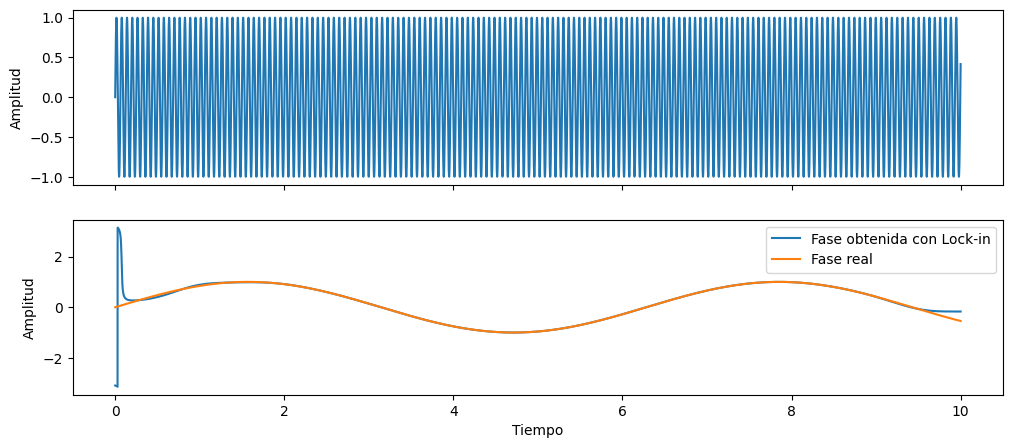
\includegraphics[width=0.9\linewidth]{Figures/31_03_2025/Lock_in}
	\caption{Comparación de fase extraída con lock-in y original para una modulación sinusoidal de la fase.}
	\label{fig:lockin}
\end{figure}


\subsection*{La simulación}
Para estudiar el comportamiento del circuito se simuló mediante \textit{Python}, resolviendo la ecuación diferencial con \textit{Odeint} de \textit{Scipy.integrate} para distintos parámetros y $l(t)$. El código final que toma la lista de parámetros y la función de alturas en función del tiempo es:

\begin{lstlisting}
from scipy.integrate import odeint
	
def measured_l(ts, l, C0, C, R, L, V=5, cutoff_freq=1):
	omega = 1 / np.sqrt(C0 * L)
	Q = (1 / R) * np.sqrt(L / C0)
	
	def C_(t):
		return C0 + C * l(t)
	
	def dXdt(X, t):
		i, didt = X
		didt2 = V * np.cos(omega * t) - R / L * didt - 1 / (C_(t) * L) * i
		return [didt, didt2]
	
	y0 = [0, 0]
	sol = odeint(dXdt, y0, ts)
	current = sol[:, 0]  
	
	_, phi_t_extracted = lock_in(current, omega, fs = 1 / (ts[1] - ts[0]), 
				    cutoff_freq=cutoff_freq)
	
	unwrapped = np.unwrap(phi_t_extracted)
	reconstructed_heights = -C0 * unwrapped / (Q * C)
	
	return reconstructed_heights
\end{lstlisting}

Devolviendo al final la lista de las alturas reconstruídas. A continuación algunas de las pruebas realizadas.


\begin{figure}[!ht]
	\centering
	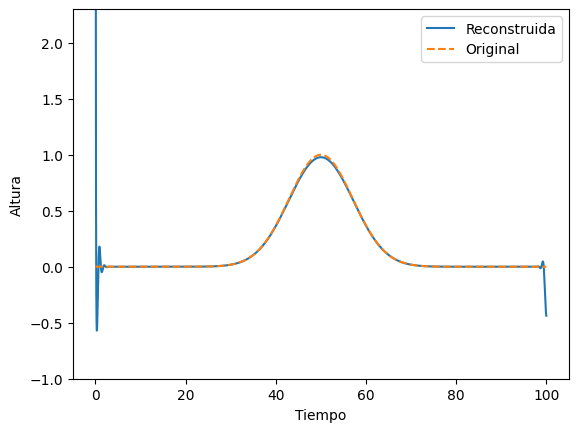
\includegraphics[width=0.45167\linewidth]{Figures/31_03_2025/Altura_gaussiana}
	\caption{Reconstrucción de alturas para una $l(t)$ Gaussiana.}
	\label{fig:alturagaussiana}
\end{figure}

En primer lugar para una $l(t)$ Gaussiana se reconstruye muy fielmente la altura original con el método propuesto. Al inicio los artefactos son por las condiciones iniciales transitorias del sistema, hasta que alcanza un estacionario.

\begin{figure}[!ht]
	\centering
	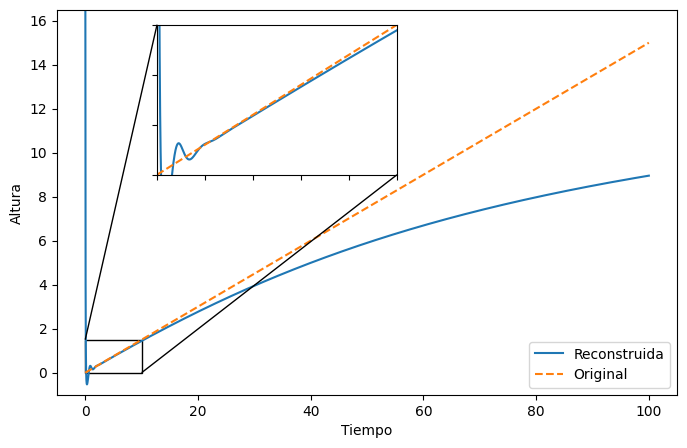
\includegraphics[width=0.45167\linewidth]{Figures/31_03_2025/Altura_lineal}
	\caption{Barrido lineal de alturas.}
	\label{fig:alturalineal}
\end{figure}


Luego con una lineal para estudiar sus límites, podemos ver que para $l$'s bajos se comporta linealmente, pero luego satura. Esto será cuando $C_0 \sim C'l$. Con lo cual si hacemos más pequeño $C'$ mejorará el rango de funcionamiento, aunque disminuirá la sensitividad, ya que es proporcional al error en fase del lock-in (que está fijo) por $C'$.

\begin{figure}[!ht]
	\centering
	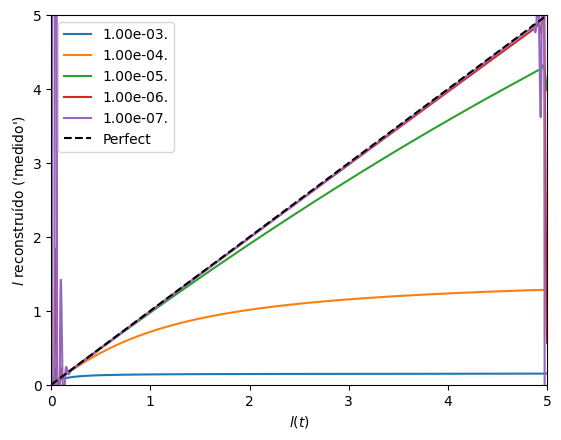
\includegraphics[width=0.4516\linewidth]{Figures/31_03_2025/Altura_lineal_varios_Cp}
	\caption{Comparación para el mismo barrido con distintos $C'$.}
	\label{fig:alturalinealvarioscp}
\end{figure}

\subsection*{Valores reales}
Siguiendo los valores usados por \cite{gordillozavaletaNonpropagatingHydrodynamicSolitons2012} se propone usar $R\sim 1$ k$\Omega$, $L=22$ mH, $C_0 = 250$ pF y $C'\sim10$ pF/mm. Estos parámetros dan una frecuencia $\omega\sim10^{5}$ Hz o $f\approx60$ kHz. Analizamos el comportamiento para una señal $l(t)$ de frecuencia $\omega=1$ kHz y amplitud 1 mm.

\begin{figure}[!ht]
	\begin{minipage}[c]{0.5\textwidth}
		\begin{subfigure}{\textwidth}
			\centering
			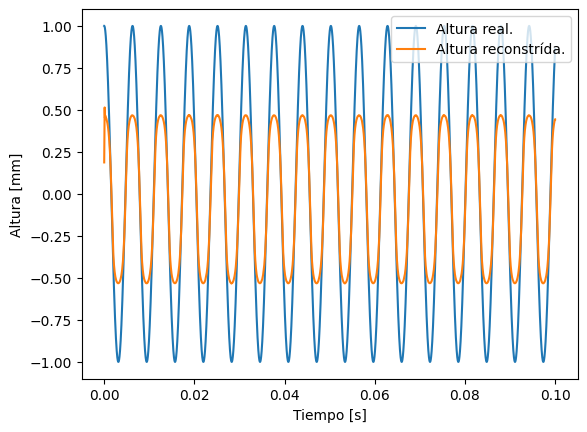
\includegraphics[width=0.8\textwidth]{Figures/31_03_2025/Barrido_valores_reales}
			\captionsetup{width=0.8\textwidth}
			\subcaption{}
		\end{subfigure}
	\end{minipage}\begin{minipage}[c]{0.49\textwidth}
		\begin{subfigure}{\textwidth}
	    	\centering
			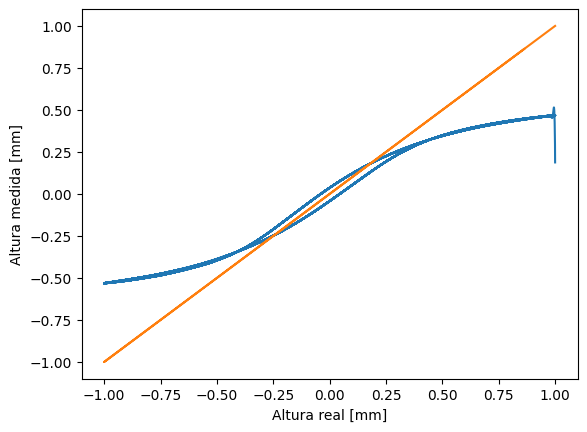
\includegraphics[width=0.8\textwidth]{Figures/31_03_2025/Barrido_valores_reales_histeresis}
			\captionsetup{width=0.8\textwidth}
			\subcaption{}
		\end{subfigure}
    \end{minipage}
	\caption{Barrido de alturas. A la izquierda la evolución temporal y a la derecha la altura reconstruída contra la original.}
	\label{fig:Barrido_alturas}
\end{figure}
	
Podemos notar que satura cerca de 0.25 mm y que a esta frecuencia de señal hay histéresis.	Si aumentamos $C_0$, suponiendo $C'$ fija, podemos conseguir aumentar el rango de validez hasta 10 mm y evitar la histéresis a 100 Hz, aunque querríamos frecuencias más altas. Esto se puede lograr también disminuyendo $Q_F$ al disminuir $L$ o aumentar $R$ por ejemplo.

\begin{figure}[!ht]
	\begin{minipage}[c]{0.5\textwidth}
		\begin{subfigure}{\textwidth}
			\centering
			\includegraphics[width=0.8\textwidth]{Figures/31_03_2025/Barrido_valores_reales_mejor_más_rango}
			\captionsetup{width=0.8\textwidth}
			\subcaption{}
		\end{subfigure}
	\end{minipage}\begin{minipage}[c]{0.49\textwidth}
		\begin{subfigure}{\textwidth}
			\centering
			\includegraphics[width=0.8\textwidth]{Figures/31_03_2025/Barrido_valores_reales_mejor_histéresis}
			\captionsetup{width=0.8\textwidth}
			\subcaption{}
		\end{subfigure}
	\end{minipage}
	\caption{Barrido de alturas. A la izquierda la evolución temporal y a la derecha la altura reconstruída contra la original.}
	\label{fig:Barrido_alturas_mejor}
\end{figure}

Esto último es para $C'=3\times10^{-8}$ F/m y $C_0=160\times10^{-10}$ F. Habrá que probar experimentalmente qué rango de valores funcionan mejor y si hay más juego antes de que sature.

\clearpage
\section{Fabricación del sensor.}
Por último se empezó con el diseño del sensor. Éste constará de una carcasa externa para integridad estructural impresa en 3D, diseñada con Blender como se muestra a continuación (primer prototipo).

\begin{figure}[!ht]
	\begin{minipage}[c]{0.5\textwidth}
		\begin{subfigure}{\textwidth}
			\centering
			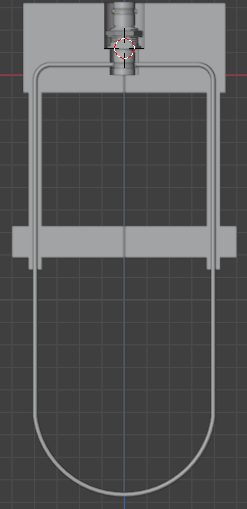
\includegraphics[width=0.678\textwidth]{Figures/31_03_2025/Modelo_3D_1}
			\captionsetup{width=0.8\textwidth}
			\subcaption{}
		\end{subfigure}
	\end{minipage}\begin{minipage}[c]{0.49\textwidth}
		\begin{subfigure}{\textwidth}
			\centering
			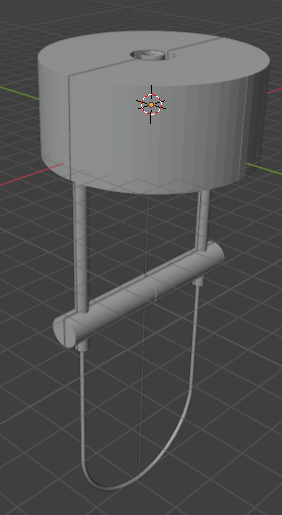
\includegraphics[width=0.76878\textwidth]{Figures/31_03_2025/Modelo_3D_2}
			\captionsetup{width=0.8\textwidth}
			\subcaption{}
		\end{subfigure}
	\end{minipage}
	\caption{Dos vistas del prototipo inicial. Entero y corte.}
	\label{fig:Modelo_3D_prototipo_inicial}
\end{figure}

Se suelda el cable de cobre a un conector BNC hembra dentro de la carcasa. Además se coloca soldado cable de acero a la carcasa exterior del BNC (a Tierra) que se conectan al alambre por abajo (aislado eléctricamente).


